\let\negmedspace\undefined
\let\negthickspace\undefined
\documentclass[journal,12pt,twocolumn]{IEEEtran}
\usepackage{gensymb}
\usepackage{polynom}
\usepackage{amssymb}
\usepackage[cmex10]{amsmath}
\usepackage{amsthm}
\usepackage{stfloats}
\usepackage{bm}
\usepackage{longtable}
\usepackage{enumitem}
\usepackage{mathtools}
\usepackage{tikz}
\usepackage[breaklinks=true]{hyperref}
\usepackage{listings}
\usepackage{color}                                            
\usepackage{array}                                            
\usepackage{longtable}                                        
\usepackage{calc}                                             
\usepackage{multirow}                                         
\usepackage{hhline}                                           
\usepackage{ifthen}                                           
\usepackage{lscape}     
\usepackage{tfrupee}
\DeclareMathOperator*{\Res}{Res}
\DeclareMathOperator*{\equals}{=}
\hyphenation{op-tical net-works semi-conduc-tor}
\def\inputGnumericTable{}                                 
\lstset{
frame=single, 
breaklines=true,
columns=fullflexible
}
\begin{document}
\newtheorem{theorem}{Theorem}[section]
\newtheorem{problem}{Problem}
\newtheorem{proposition}{Proposition}[section]
\newtheorem{lemma}{Lemma}[section]
\newtheorem{corollary}[theorem]{Corollary}
\newtheorem{example}{Example}[section]
\newtheorem{definition}[problem]{Definition}
\newcommand{\BEQA}{\begin{eqnarray}}
\newcommand{\EEQA}{\end{eqnarray}}
\newcommand{\define}{\stackrel{\triangle}{=}}
\newcommand*\circled[1]{\tikz[baseline=(char.base)]{
\node[shape=circle,draw,inner sep=2pt] (char) {#1};}}
\bibliographystyle{IEEEtran}
\providecommand{\mbf}{\mathbf}
\providecommand{\pr}[1]{\ensuremath{\Pr\left(#1\right)}}
\providecommand{\qfunc}[1]{\ensuremath{Q\left(#1\right)}}
\providecommand{\sbrak}[1]{\ensuremath{{}\left[#1\right]}}
\providecommand{\lsbrak}[1]{\ensuremath{{}\left[#1\right.}}
\providecommand{\rsbrak}[1]{\ensuremath{{}\left.#1\right]}}
\providecommand{\brak}[1]{\ensuremath{\left(#1\right)}}
\providecommand{\lbrak}[1]{\ensuremath{\left(#1\right.}}
\providecommand{\rbrak}[1]{\ensuremath{\left.#1\right)}}
\providecommand{\cbrak}[1]{\ensuremath{\left\{#1\right\}}}
\providecommand{\lcbrak}[1]{\ensuremath{\left\{#1\right.}}
\providecommand{\rcbrak}[1]{\ensuremath{\left.#1\right\}}}
\theoremstyle{remark}
\newtheorem{rem}{Remark}
\newcommand{\sgn}{\mathop{\mathrm{sgn}}}
\providecommand{\fourier}{\overset{\mathcal{F}}{ \rightleftharpoons}}
\providecommand{\system}{\overset{\mathcal{H}}{ \longleftrightarrow}}
\newcommand{\solution}{\noindent \textbf{Solution: }}
\newcommand{\cosec}{\,\text{cosec}\,}
\providecommand{\dec}[2]{\ensuremath{\overset{#1}{\underset{#2}{\gtrless}}}}
\newcommand{\myvec}[1]{\ensuremath{\begin{pmatrix}#1\end{pmatrix}}}
\newcommand{\mydet}[1]{\ensuremath{\begin{vmatrix}#1\end{vmatrix}}}
\makeatletter
\@addtoreset{figure}{problem}
\makeatother
\let\StandardTheFigure\thefigure
\let\vec\mathbf
\def\putbox#1#2#3{\makebox[0in][l]{\makebox[#1][l]{}\raisebox{\baselineskip}[0in][0in]{\raisebox{#2}[0in][0in]{#3}}}}
\def\rightbox#1{\makebox[0in][r]{#1}}
\def\centbox#1{\makebox[0in]{#1}}
\def\topbox#1{\raisebox{-\baselineskip}[0in][0in]{#1}}
\def\midbox#1{\raisebox{-0.5\baselineskip}[0in][0in]{#1}}
\title{Assignment-1}
\author{ Aniket Satpute (CS21BTECH11056)}
\graphicspath{{figure/}}
\maketitle
\begin{abstract}
ICSE Class 10 Maths 2017 Q.8(a)
\end{abstract}

% the text begins here

Question 8\\

(a)	Calculate the mean of the following distribution using step deviation method.\\

\begin{table}[h!]
\center
\resizebox{\columnwidth}{!}
{
\begin{tabular}{|c|c|c|c|c|c|c|}
\hline
Marks & 0-10 & 10-20 & 20-30 & 30-40 & 40-50 & 50-60 \\
\hline
Number of Students & 10 & 9 & 25 & 30 & 16 & 10 \\
\hline
\end{tabular}
}
\end{table}
\textbf{ Solution : }\\
Here, In the Assignment-1-Solution-Table :\\
\begin{equation*}
Assumed mean : A=25
\end{equation*}
\begin{equation*}
Mid-value : x
\end{equation*}
\begin{equation*}
class-size : i
\end{equation*}
\begin{equation*}
t = \frac{(x-A)}{i}
\end{equation*}
\begin{table}[h!]
\center
\resizebox{\columnwidth}{!}
{
\begin{tabular}{|c|c|c|c|c|}
\hline
Class-Interval & Mid-value & No of Students & t & ft\\
(Marks) & (x) & (f) & & \\
\hline
0-10 & 5 & 10 & -2 & -20 \\
\hline
10-20 & 15 & 9 & -1 & -9\\
\hline
20-30 & 25 & 25 & 0 & 0\\
\hline
30-40 & 35 & 30 & 1 & 30\\
\hline
40-50 & 45 & 16 & 2 & 32\\
\hline
50-60 & 55 & 10 & 3 & 30\\
\hline
 	&		 & 		$ 	\sum f = 100$ 		 &	 &	$ \sum ft = 63$		\\
 \hline
\end{tabular}
}
\end{table}
From the Solution Table :\\
\begin{equation*}
\sum f = 100
\end{equation*}
\begin{equation*}
\sum ft = 63
\end{equation*}
\begin{align*}
Mean & = A + \frac{ \sum ft }{\sum f} * i\\
     & = 25 + \frac{63}{100} * 10\\
     & = 25 + 6.3\\
     & = 31.3\\\
\end{align*}
Hence , Mean of given data is 31.3\\
\textbf{Solution(Vector Operations)}\\
By given Data :\\
\begin{table}[h!]
\center
{
\begin{tabular}{|c|c|}
\hline
$\vec{F}$ & frequency vector\\
\hline
$\vec{X}$ & mid-value vector\\
\hline
i &  10\\
\hline
$\vec{T}$ &  $(\vec{X}-\vec{A})/i$\\
\hline
$\vec{F}^{T}\vec{T}$ &  Dot-product\\
\hline
\end{tabular}
}
\end{table}
\begin{align}
\vec{F} & = 
\myvec{10 \\ 9 \\ 25 \\ 30 \\ 16 \\ 10}
\end{align}
\begin{align}
\vec{X} & = 
\myvec{5 \\ 15 \\ 25 \\ 35 \\ 45 \\ 55}
\end{align}
\begin{align}
\vec{A} = 
\myvec{25\\25\\25\\25\\25\\25}
\end{align}
\begin{align}
\vec{T} & =
\myvec{-2 \\ -1 \\ 0 \\ 1 \\ 2 \\ 3 }
\end{align}
\begin{align}
\vec{F}^{T}\vec{T}  & =\myvec{10 & 9 & 25 & 30 & 16 & 10}\myvec{-2\\-1\\0\\1\\2\\3}\\ 
                    & = 63
\end{align}
\begin{align}
\sum f & = F^{T} \myvec{1\\1\\1\\1\\1\\1}\\
	   & = \myvec{10 & 9 & 25 & 30 & 16 & 10}\myvec{1\\1\\1\\1\\1\\1}\\
       & = 63
\end{align}
\begin{align}
Mean & = A + \frac{ \vec{F}^{T}\vec{T} }{\sum f} * i\\
     & = 25 + \frac{63}{100} * 10\\
     & = 25 + 6.3\\
     & = 31.3
\end{align}
\textbf{Mean Deviation Method By Graph :}
\begin{figure}[h]
\centering
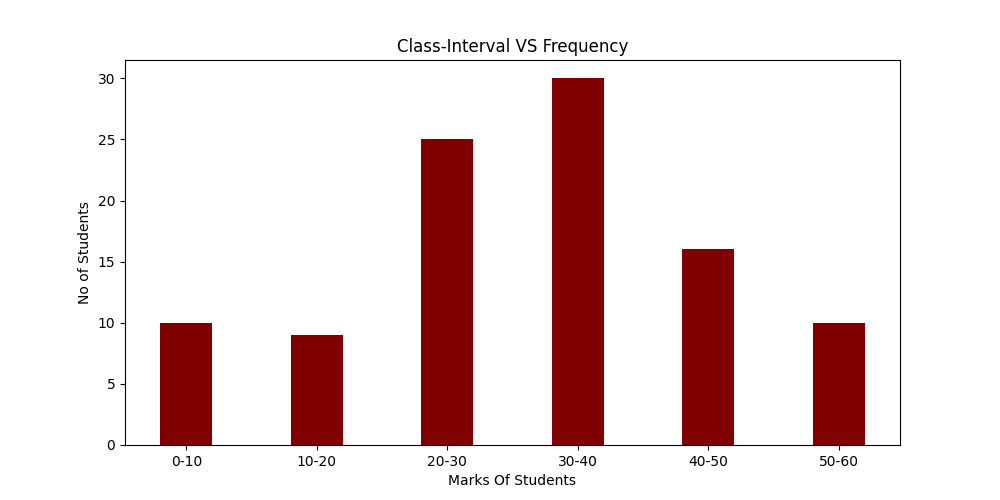
\includegraphics[width=\columnwidth]{Assig-1-figure.png}
\caption{Mean Deviation Method}
\label{Fig1}
\end{figure}\\
In the graph we see distribution of Number of students against the marks of students.\\In the Mean-Deviation-Method we assume a mean in this case the Assumed-Mean (\textbf{A}) is 25 , then we define the term 't' which is measure of deviation of any class interval wrt to the Assumed-Mean \\Then we calculate the summation of this deviation multiplied by the frequency of that class to obtain overall deviation of the data \\As we get the overall deviation to get the actual mean we add the mean of the deviation of each class-Interval to the Assumed-Mean.to calculate the mean of deviation we divide the summation of deviation by summation of frequency and multiply by classlength(\textbf{i}) (As in t is divided) . In this way we get the Mean of the Data.
\end{document}